\chapter{Wertannahme stetiger Funktionen}
\Mark{Chapter 3.2}
\begin{fsatz}
Die Funktion $f$: $D \ra \R$ sei stetig in $x_0$ und es gelte $f(x_0) > 0 (f(x_0)< 0)$. Dann gibt es eine Umgebung $U(x_0)$ von $x_0$ (\ac{d.h.} $\exists \delta > 0 U_{\mathbf{\delta}} (x_0) (x_0 - \delta, x_0 + \delta)$) so dass $\forall x \in U_{\delta} (x_0) \cap D$: $f(x) > 0$ ($f(x) < 0$).
\Mark{Satz 3.5}
\end{fsatz}

\begin{fbeweis}
Sei $f(x_0) > 0$ und $f$ in $x_0$ stetig. Nach \ac{Def.} der Stetigkeit gilt $\forall \epsilon > 0$ $\exists \delta (\epsilon, x_0) > 0$ so dass $\ub{\forall x \in D \tx{ mit } \betrag{x - x_0} < \delta}{\Lra x \in U_{\delta} (x_0)}$ \Ra $\ub{\betrag{f(x) - f(x_0)} < \epsilon}{\Lra f(x_0) - \epsilon < f(x) < f(x_0) + \epsilon}$
\begin{align*}
&\epsilon \ceq \frac{1}{2} f(x_0) > 0\\
&f(x) > f(x_0) - \epsilon = f(x_0) - \frac{1}{2} f(x_0) = \rac{1}{2} f(x_0)
\end{align*} \qed
\end{fbeweis}

\begin{fsatz}[Zwischenwertsatz]
\label{satz:Wertannahme_stetiger_Funktionen_S3_6}
Die Funktion $f$: $[a, b] \ra \R$ sei auf dem ganzen Intervall $[a, b]$ stetig und $f(a) \mal f(b) < 0$. Dann gibt es ein $\xi \in (a, b)$ mit $f(\xi) = 0$
\begin{center}
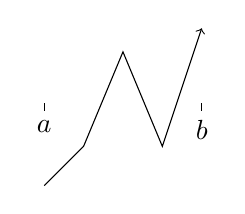
\begin{tikzpicture}
\tikzcoor[x][]{3.5}{1.5}

\foreach \x/\y in{1/a,3/b}
	\draw (\x,-0.05) node[below] {$\y$} -- (\x,0.05);

\draw[->] (1,-1) -- (1.5,-0.5) -- (2, 0.7) -- (2.5,-0.5) -- (3,1);
\end{tikzpicture}
\end{center}
\Img{MA2-23.04.2009-IMG-1}

\Mark{Satz 3.6}
\end{fsatz}

\begin{fbeweis}[Konstruktiver Beweis]
Sei \ac{OBdA} $f(a) < 0$, $f(b) > 0$\\
Folge von Intervallen $([x_n, y_n])_{n \in \N}$
\begin{enumerate}
\item $[x_n, y_n] \subset [x_{n - 1}, y_{n - 1}]$
\item $y_n - x_n = 2^{-n} (b -a)$
\item $f(x_n) \klgl 0$, $f(y_n > 0)$
\end{enumerate}
\begin{description}
\item[(IA)] $[x_0, y_0] = [a, b]$ erf�llt Bedingungen 2/3
\item[(IS)] $[x_n, y_n]$ sei bereits definiert und erf�lle die drei Bedingungen\\
		\[m \ceq \frac{x_n + y_n}{2}\]
		\begin{description}
		\item[Fall 1 $f(m) \klgl 0$] $[x_{n + 1}, y_n{n + 1}] = [m, y_n]$
		\item[Fall 2 $f(m) > 0$] $[x_{n + 1}, y_{n + 1}] = [x_n, m]$
		\end{description}
		Die drei Bedingungen sind f�r beide F�lle erf�llt.
		\begin{itemize}
		\item $(x_n)_{n \in \N_0}$ ist eine monoton wachsende und durch $b$ nach oben beschr�nkte Folge.
				\begin{itemize}[label=\Ra]
				\item $(x_n)_{n \in \N_0}$ ist konvergent
				\end{itemize}

		\item $(y_n)_{n \in \N_0}$ ist eine monoton fallende und durch $a$ nach unten beschr�nkte Folge.
				\begin{itemize}[label=\Ra]
				\item $(x_n)_{n \in \N_0}$ ist konvergent
				\end{itemize}
		\end{itemize}

		wegen 2) gilt:
		\begin{align*}
		&\lim_{n \ra \un} (y_n - x_n) = \lim_{n \ra \un} 2^{-n} (b - a) = 0\\
		=& \lim_{n \ra \un} y_n - \lim_{n \ra \un} x_n\\
		\Ra & \lim_{n \ra \un} (y_n) = \lim_{n \ra \un} (x_n) \eqc \xi
		\end{align*}
		Da $f$ stetig ist gilt:
		\begin{align*}
		\ub{\lim_{n \ra \infty} f(y_n)}{\ub{\lim_{y \searrow \xi} f(y)}{\grgl 0}} = f(\xi) = \ub{lim_{n \ra \infty} f(x_n)}{\ub{\lim_{x \nearrow \xi} f(x)}{\klgl 0}}
		\Ra f(\xi) = 0
		\end{align*} \qed
\end{description}
\end{fbeweis}

\begin{beispiel}
$f(x) = x^3 - 1$, $[a, b] = [0, 2]$
\begin{enumerate}[label=\arabic*), start=0]
\item $[x_0, y_0] = [0, 2]$
\item $f(1) = -1 \stack{\tx{Fall 1}}{\Ra} [x_1, y_1] = [1, 2]$
\item $f \rkl{\frac{3}{2}} = \frac{27}{8} - \frac{16}{8} = \frac{11}{8} > 0 \stack{\tx{Fall 2}}{\Ra} [x_2, y_2] = \eklamm{1, \frac{3}{2}}$
\item $f \rkl{\frac{5}{4}} = \frac{125}{64} - \frac{128}{64} = - \frac{3}{64} < 0 \stack{\tx{Fall 1}}{\Ra} \eklamm{\frac{5}{4}, \frac{3}{2}}$\\
		$\vdots$
\end{enumerate}
$M = \frac{1 + 2}{2}$
\end{beispiel}

\begin{bemerkung}
\mbox{}\par
\begin{enumerate}
\item Das Konstruktionsverfahren im obigen Beweis nennt man auch Intervallhalbierungsmethode \ac{bzw.} Bisektionsmethode.
\item Der Satz \vref{satz:Wertannahme_stetiger_Funktionen_S3_6} Kann erweitert werden zur Aussage, dass jeder Wert zwischen $f(a)$ und $f(b)$ angenommen wird.
		\Mark{MA-23.04.2009-IMG-2}
\end{enumerate}
\end{bemerkung}

\section{Aufgabe 3.3}
Zeigen Sie:
\begin{enumerate}[label=\alph*)]
\item Es gibt mindestens einen Schnittpunkt der beiden Funktionen $f$: $[0, \un) \ra \R$, $x \mapsto f(x) = x^2$ und $g$: $[0, \un) \ra \R$, $x \mapsto g(x) = 2$.
\item Es gibt mindestens eine L�sung der Gleichung $x^2 = \cosx{}$.
\end{enumerate}
\Todo{Ref zur L�sung}

\begin{fsatz}[Existenz von Maximum/Minimum]
\label{satz:Wertannahme_stetiger_Funktionen_3_7}
Sei $f$: $D \ra \R$ stetig. Dann nimmt $f$ auf einem Intervall $[a, b] \subseteq D$ sein Maximum und sein Minimum an.\\
Daher $\exists \underline{x}, \overline{x} \in [a, b]$ mit\\
\[\forall x \in [a, b]:~ f(x) \klgl f(x) \klgl f(\overline{x})\]
\Mark{Satz 3.7}
\end{fsatz}

\begin{fbeweis}
-
\end{fbeweis}

\begin{bemerkung}
\mbox{}\par
\begin{enumerate}
\item Es ist wichtig, dass das Intervall abgeschlossen ist.
		\begin{beispiel}[F�r Probleme bei offenen Intervallen]
		\begin{align*}
		f:~(0, 1) \ra &\R\\
		x \mapsto &\frac{1}{x}
		\end{align*}
		\Mark{MA-23.04.2009-IMG-3}
		\end{beispiel}

\item Es kann auch mehrere oder gar $\un$-viele Maxima/Minima geben
		\begin{beispiel}
		\begin{align*}
		f:~(0, 4\pi) \ra &\R\\
		x \mapsto &\cosx{}
		\end{align*}
		\Mark{MA-23.04.2009-IMG-4}
		\[\overline{x} \in \gklamm{0, 2\pi, 4\pi}, \underline{x} \in \gklamm{\pi, 3\pi}\]
		\end{beispiel}

		\begin{beispiel}
		\begin{align*}
		f:~(-1, 2) \ra &\R\\
		x \mapsto &f(x) = \begin{cases}0 & \tx{f�r } -1 \klgl x \klgl 0\\x & \tx{f�r } 0 < x < 1\\1 & \tx{f�r } 1 \klgl x \klgl 2\end{cases}
		\end{align*}
		\end{beispiel}
		\Mark{MA-23.04.2009-IMG-5}

\item Falls $f$ zudem differenzierbar ist, kann man die Orte der Maxima/Minima bestimmen
\end{enumerate}
\end{bemerkung}

\section{L�sungen}
\subsection{Aufgabe 3.3}
\begin{enumerate}[label=\alph*)]
\item $\exists$ Schnittpunkt von $f(x) = x^2$ und $g(x) = 2$ in $[0, \un)$\\
		\Lra $\exists x \in [0, \un)$: $f(x) = 2$
		\begin{description}
		\item[Variante 1] Anpassen des Beweises von Satz \vref{satz:Wertannahme_stetiger_Funktionen_S3_6} auf den Zwischenwert $2$ statt $0$.\\
				Folge von Intervallen mit $1, 2$ wie gehabt.\\
				\begin{enumerate}[label=\arabic*), start=3]
				\item $f(x_n) \klgl 2$, $f(y_n) > 2$
				\begin{description}
				\item[(IA)] $[x_0, y_0] = [0, 2]$ $f(0) = 0 < 2$, $f(2) = 4 > 2$
				\item[(IS)] \dots
						\begin{description}
						\item[Fall 1] $f(m) \klgl 2$
						\item[Fall 2] $f(m) > 2$
						\end{description}
				\end{description}
				\end{enumerate}

		\item[Variante 2] \ac{z.z.} $\exists x \in [0, \un)$ mit $x^2 = 2$ ($\Lra x^2 - 2 = 0$)
				\[h(x) = x^2 - 2\]
				da $h(0) = -2 < 0$, $h(2) = 2 > 0$, $h$ stetig besagt das Zwischenwertsatz, dass ein $\xi \in [0, 2]$ existiert mit $h(\xi) = 0$ ($\Lra f(\xi) = g(\xi) = 2$)
		\end{description}

\item $\exists x \in \R$: $x^2 = \cosx{}$ ($\Lra x^2 - \cosx{} = 0$)
		\begin{align*}
		&h(x) = x^2 - \cosx{}, [a, b] = \eklamm{0, \frac{\pi}{2}}\\
		&h(0) = -1 < 0, h \rkl{\frac{\pi}{2}} = \frac{\pi^2}{4} > 0
		\end{align*}
		Zwischenwertsatz auf $h$ anwenden.
\end{enumerate}
\Todo{Ref zur Aufgabe}
